% Options for packages loaded elsewhere
\PassOptionsToPackage{unicode}{hyperref}
\PassOptionsToPackage{hyphens}{url}
%
\documentclass[
]{article}
\usepackage{amsmath,amssymb}
\usepackage{lmodern}
\usepackage{iftex}
\ifPDFTeX
  \usepackage[T1]{fontenc}
  \usepackage[utf8]{inputenc}
  \usepackage{textcomp} % provide euro and other symbols
\else % if luatex or xetex
  \usepackage{unicode-math}
  \defaultfontfeatures{Scale=MatchLowercase}
  \defaultfontfeatures[\rmfamily]{Ligatures=TeX,Scale=1}
\fi
% Use upquote if available, for straight quotes in verbatim environments
\IfFileExists{upquote.sty}{\usepackage{upquote}}{}
\IfFileExists{microtype.sty}{% use microtype if available
  \usepackage[]{microtype}
  \UseMicrotypeSet[protrusion]{basicmath} % disable protrusion for tt fonts
}{}
\makeatletter
\@ifundefined{KOMAClassName}{% if non-KOMA class
  \IfFileExists{parskip.sty}{%
    \usepackage{parskip}
  }{% else
    \setlength{\parindent}{0pt}
    \setlength{\parskip}{6pt plus 2pt minus 1pt}}
}{% if KOMA class
  \KOMAoptions{parskip=half}}
\makeatother
\usepackage{xcolor}
\usepackage[margin=1in]{geometry}
\usepackage{graphicx}
\makeatletter
\def\maxwidth{\ifdim\Gin@nat@width>\linewidth\linewidth\else\Gin@nat@width\fi}
\def\maxheight{\ifdim\Gin@nat@height>\textheight\textheight\else\Gin@nat@height\fi}
\makeatother
% Scale images if necessary, so that they will not overflow the page
% margins by default, and it is still possible to overwrite the defaults
% using explicit options in \includegraphics[width, height, ...]{}
\setkeys{Gin}{width=\maxwidth,height=\maxheight,keepaspectratio}
% Set default figure placement to htbp
\makeatletter
\def\fps@figure{htbp}
\makeatother
\setlength{\emergencystretch}{3em} % prevent overfull lines
\providecommand{\tightlist}{%
  \setlength{\itemsep}{0pt}\setlength{\parskip}{0pt}}
\setcounter{secnumdepth}{5}
\newlength{\cslhangindent}
\setlength{\cslhangindent}{1.5em}
\newlength{\csllabelwidth}
\setlength{\csllabelwidth}{3em}
\newlength{\cslentryspacingunit} % times entry-spacing
\setlength{\cslentryspacingunit}{\parskip}
\newenvironment{CSLReferences}[2] % #1 hanging-ident, #2 entry spacing
 {% don't indent paragraphs
  \setlength{\parindent}{0pt}
  % turn on hanging indent if param 1 is 1
  \ifodd #1
  \let\oldpar\par
  \def\par{\hangindent=\cslhangindent\oldpar}
  \fi
  % set entry spacing
  \setlength{\parskip}{#2\cslentryspacingunit}
 }%
 {}
\usepackage{calc}
\newcommand{\CSLBlock}[1]{#1\hfill\break}
\newcommand{\CSLLeftMargin}[1]{\parbox[t]{\csllabelwidth}{#1}}
\newcommand{\CSLRightInline}[1]{\parbox[t]{\linewidth - \csllabelwidth}{#1}\break}
\newcommand{\CSLIndent}[1]{\hspace{\cslhangindent}#1}
\usepackage{titling}
\pretitle{\begin{center} 
\includegraphics[width=2in,height=2in]{logo.jpg}\LARGE\\}
\posttitle{\end{center}}
\usepackage{listings}
\usepackage{xcolor}
\definecolor{customgreen}{rgb}{0,0.6,0}
\definecolor{customgray}{rgb}{0.5,0.5,0.5}
\definecolor{custommauve}{rgb}{0.6,0,0.8}
\lstset{ basicstyle=\small, breaklines=true, commentstyle=\color{customgreen}, firstnumber=1, frame=single, keepspaces=true, keywordstyle=\color{blue}, numbers=left, numbersep=10pt, numberstyle=\tiny\color{customgray}, rulecolor=\color{black}, showspaces=false, showstringspaces=false, showtabs=false, stepnumber=1, stringstyle=\color{custommauve}, tabsize=2,
\ifLuaTeX
  \usepackage{selnolig}  % disable illegal ligatures
\fi
\IfFileExists{bookmark.sty}{\usepackage{bookmark}}{\usepackage{hyperref}}
\IfFileExists{xurl.sty}{\usepackage{xurl}}{} % add URL line breaks if available
\urlstyle{same} % disable monospaced font for URLs
\hypersetup{
  pdftitle={AWS Machine Learning Engineer Nanodegree},
  pdfauthor={Masinde Mtesigwa Masinde},
  hidelinks,
  pdfcreator={LaTeX via pandoc}}

\title{AWS Machine Learning Engineer Nanodegree}
\author{Masinde Mtesigwa Masinde}
\date{2023-03-10}

\begin{document}
\maketitle

{
\setcounter{tocdepth}{3}
\tableofcontents
}
\newpage

\hypertarget{definition}{%
\section{Definition}\label{definition}}

\hypertarget{project-overview}{%
\subsection{Project Overview}\label{project-overview}}

Electronic Health records or Electronic Medical Records data is the data
being collected when we see a doctor, pick up a prescription at the
pharmacy, or even from a visit to the dentist.

This data is used for a variety of use-cases. From personalizing
healthcare to discovering novel drugs and treatments to helping
providers diagnose patients better and reduce medical errors.

Diabetes mellitus, or simply diabetes, is a leading non-communicable
disease (NCD) globally, almost doubling in cases since 1980. It is a
chronic illness that develops either when the pancreas are not able to
generate sufficient insulin or when the body does not utilize the
insulin produced effectively. There is no cure for this disease.
Diabetes is thought to result from a combination of genetic and
environmental factors. Several risk factors that are attributed to
diabetes include ethnicity, family history of diabetes, age, excess
weight, unhealthy diet, physical inactivity, and smoking. In addition to
this, the absence of early detection of diabetes has been known to
contribute to the development of other chronic diseases such as kidney
disease.

\hypertarget{dataset}{%
\subsection{Dataset}\label{dataset}}

This dataset is originally from the National Institute of Diabetes and
Digestive and Kidney Diseases. The objective of the dataset is to
diagnostically predict whether or not a patient has diabetes, based on
certain diagnostic measurements included in the dataset. Several
constraints were placed on the selection of these instances from a
larger database. In particular, all patients here are females at least
21 years old of Pima Indian heritage.

The datasets consists of several medical predictor variables and one
target variable, Outcome. Predictor variables includes the number of
pregnancies the patient has had, their BMI, insulin level, age, and so
on(Aamna 2023).

\hypertarget{problem-statement}{%
\subsection{Problem Statement}\label{problem-statement}}

Can you build a machine learning model to accurately predict whether or
not the patients in the dataset have diabetes or not?

\hypertarget{metrics}{%
\subsection{Metrics}\label{metrics}}

\hypertarget{auc}{%
\subsubsection{AUC}\label{auc}}

AUC is used for binary classification, multiclass classification, and
ranking problems. AUC measures the proportion of correctly ordered
objects and the capability of the model to distinguish between the
classes.

The AUC has an important statistical property: the AUC of a classifier
is equivalent to the probability that the classifier will rank a
randomly chosen positive instance higher than a randomly chosen negative
instance.(Volodkevich, n.d.)

AUC is the Area Under the ROC Curve. The best AUC = 1 for a model that
ranks all the objects right (all objects with class 1 are assigned
higher probabilities then objects of class 0). AUC for the `bad'
classifier which is working as random guessing is equal to
0.5.(Volodkevich, n.d.)

The ROC curve shows the model's ability to distinguishing between
classes.

The model which randomly assigns a class to object is a `bad' classifier
and has a diagonal ROC curve. The better is the classifier, the higher
is the ROC curve. The ROC curve is plotted with TPR, True Positive Rate,
on the y-axis against the FPR, False Positive Rate, on the x-axis. The
curve also could be interpreted in terms of Sensitivity and Specificity
of the model with Sensitivity on the y-axis and (1-Specificity) on the
x-axis.

Building and visualizing the ROC curve could be used to measure
classification algorithm performance with different probability
boundaries and select the probability boundary required to achieve the
specified false-positive or false-negative rate.(Volodkevich, n.d.)

\hypertarget{analysis}{%
\section{Analysis}\label{analysis}}

Data was stored in AWS S3 cloud service.

\begin{lstlisting}[language=python]
train_file = "train.csv"
train.to_csv(train_file, index=False)
train_s3_path = session.upload_data(train_file, key_prefix="{}/data".format(prefix))

test_file = "test.csv"
test.to_csv(test_file, index=False)
test_s3_path = session.upload_data(test_file, key_prefix="{}/data".format(prefix))


X_test_file = "X_test.csv"
X_test.to_csv(X_test_file, index=False)
X_test_s3_path = session.upload_data(X_test_file, key_prefix="{}/data".format(prefix))
\end{lstlisting}

\hypertarget{data-exploration}{%
\subsection{Data Exploration}\label{data-exploration}}

\textbf{DataFrame.describe()} method generates descriptive statistics
that summarize the central tendency, dispersion and shape of a dataset's
distribution, excluding NaN values. This method tells us a lot of things
about a dataset. One important thing is that the describe() method deals
only with numeric values. It doesn't work with any categorical values.
So if there are any categorical values in a column the describe() method
will ignore it and display summary for the other columns unless
parameter include=``all'' is passed.

\begin{itemize}
\tightlist
\item
  count tells us the number of NoN-empty rows in a feature.
\item
  mean tells us the mean value of that feature.
\item
  std tells us the Standard Deviation Value of that feature.
\item
  min tells us the minimum value of that feature.
\item
  25\%, 50\%, and 75\% are the percentile/quartile of each features.
  This quartile information helps us to detect Outliers.
\item
  max tells us the maximum value of that feature.
\end{itemize}

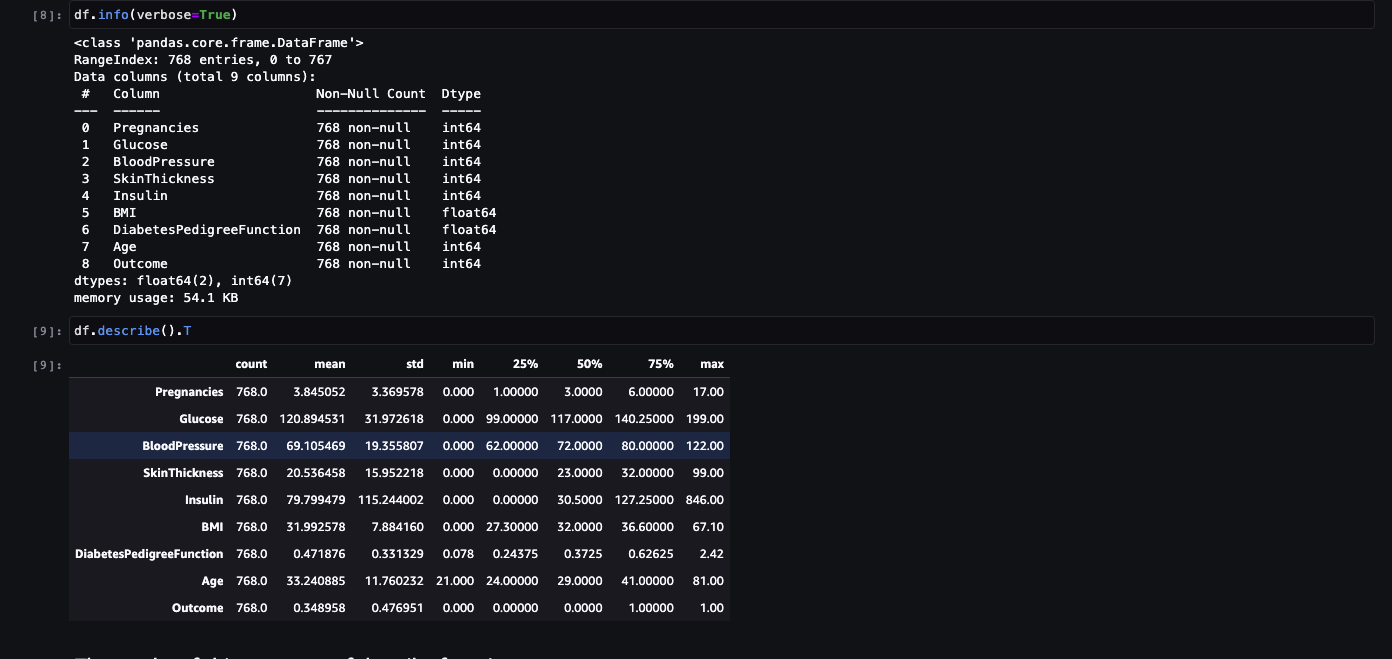
\includegraphics{describe.png} \textbf{The results of this summary of
describe function.}

There are some value of below listed columns have zero minimum, the
value of zero does indicates missing value.

Following columns or variables have an invalid zero value:

\begin{itemize}
\tightlist
\item
  Glucose
\item
  BloodPressure
\item
  SkinThickness
\item
  Insulin
\item
  BMI
\end{itemize}

\hypertarget{exploratory-visualization}{%
\subsection{Exploratory Visualization}\label{exploratory-visualization}}

\hypertarget{clean-data-distribution}{%
\subsubsection{Clean Data Distribution}\label{clean-data-distribution}}

A left-skewed distribution has a long left tail. Left-skewed
distributions are also called negatively-skewed distributions. That's
because there is a long tail in the negative direction on the number
line. The mean is also to the left of the peak.

\begin{figure}
\centering
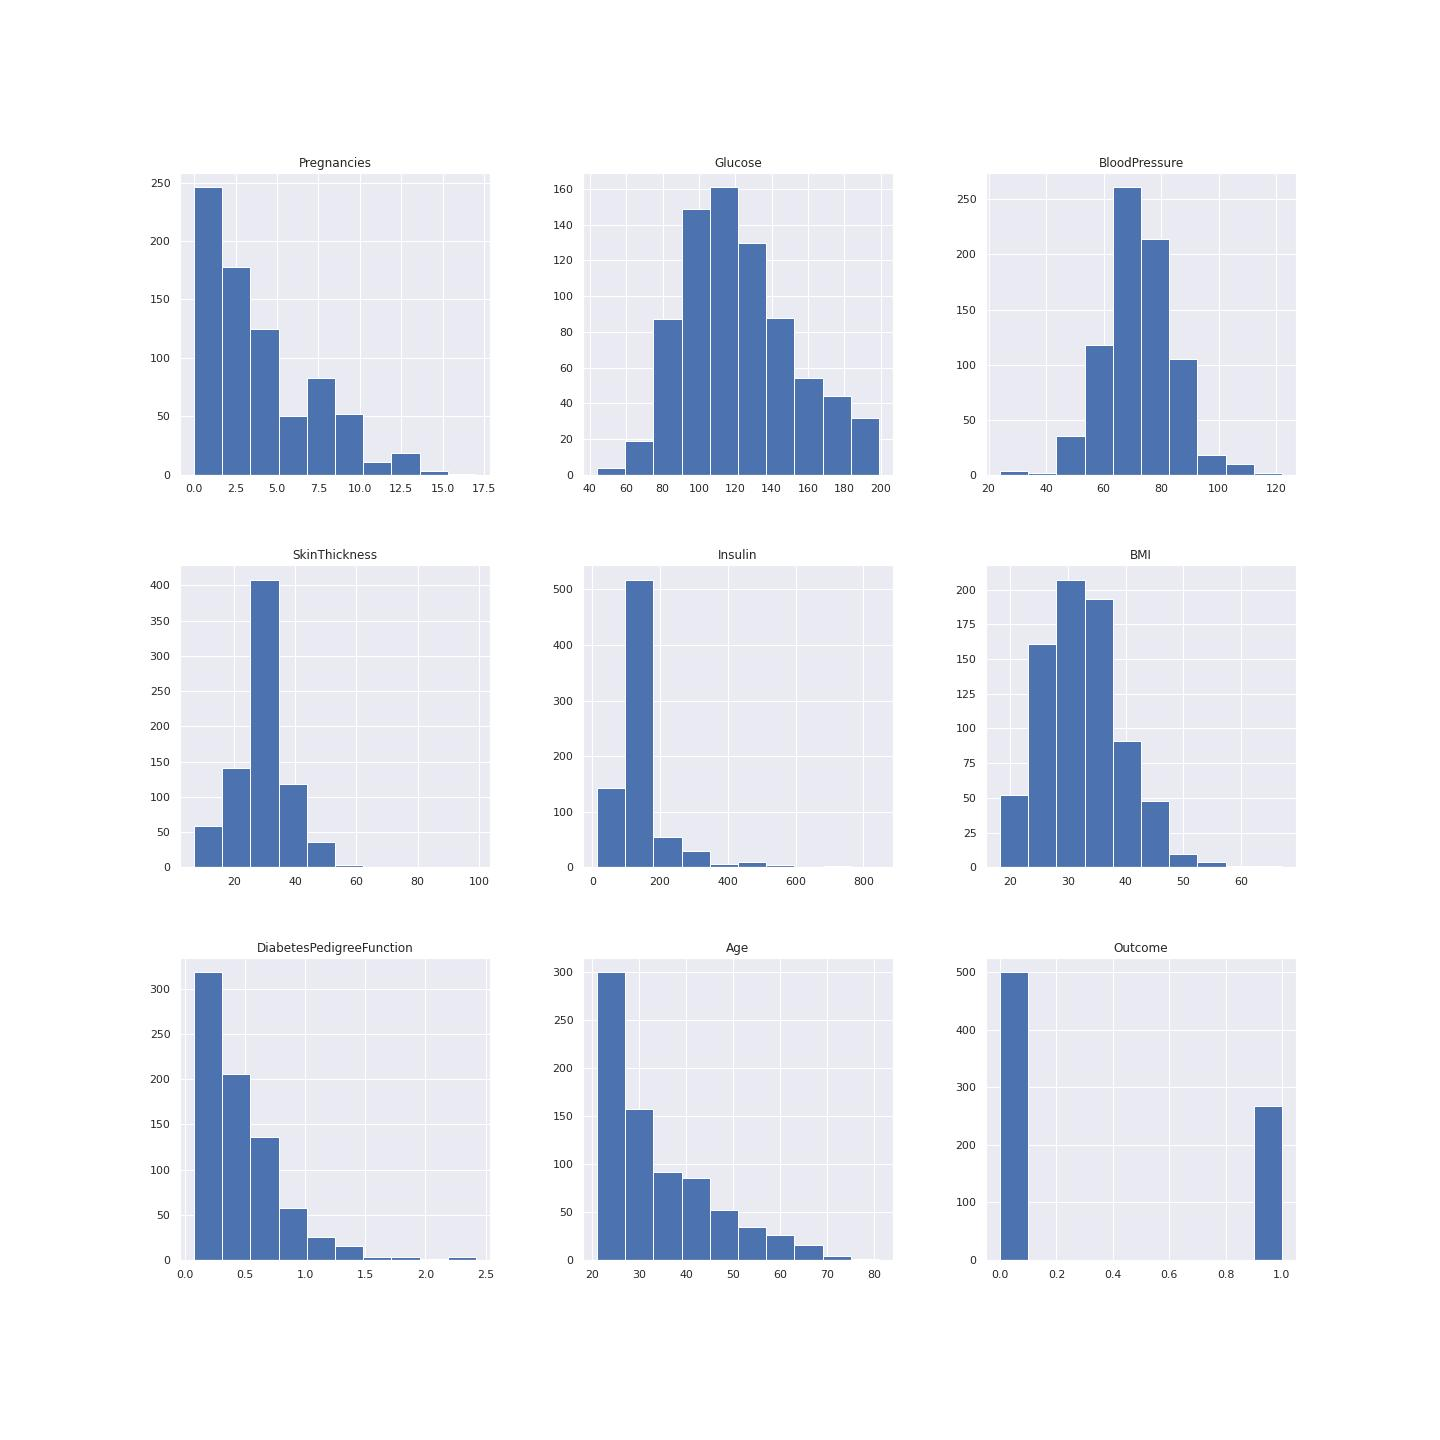
\includegraphics{clean.jpg}
\caption{Clean Data Distribution}
\end{figure}

Aright-skewed distribution has a long right tail. Right-skewed
distributions are also called positive-skew distributions. That's
because there is a long tail in the positive direction on the number
line. The mean is also to the right of the peak.

\hypertarget{correlation-visualisation}{%
\subsubsection{Correlation
visualisation}\label{correlation-visualisation}}

Heatmap is good method to visualize correlation between features. This
heatmap helps to know the following pairs had a positive correlation
coeffiecient between them as compared to other parameters.

\begin{itemize}
\tightlist
\item
  Pregnancies and age
\item
  Insulin and Skin thickness
\item
  BMI and Skin thickness
\item
  Insulin and Glucose
\end{itemize}

Glucose and BMI values are related the most. This indicates the two
parameters need special attention.

\begin{figure}
\centering
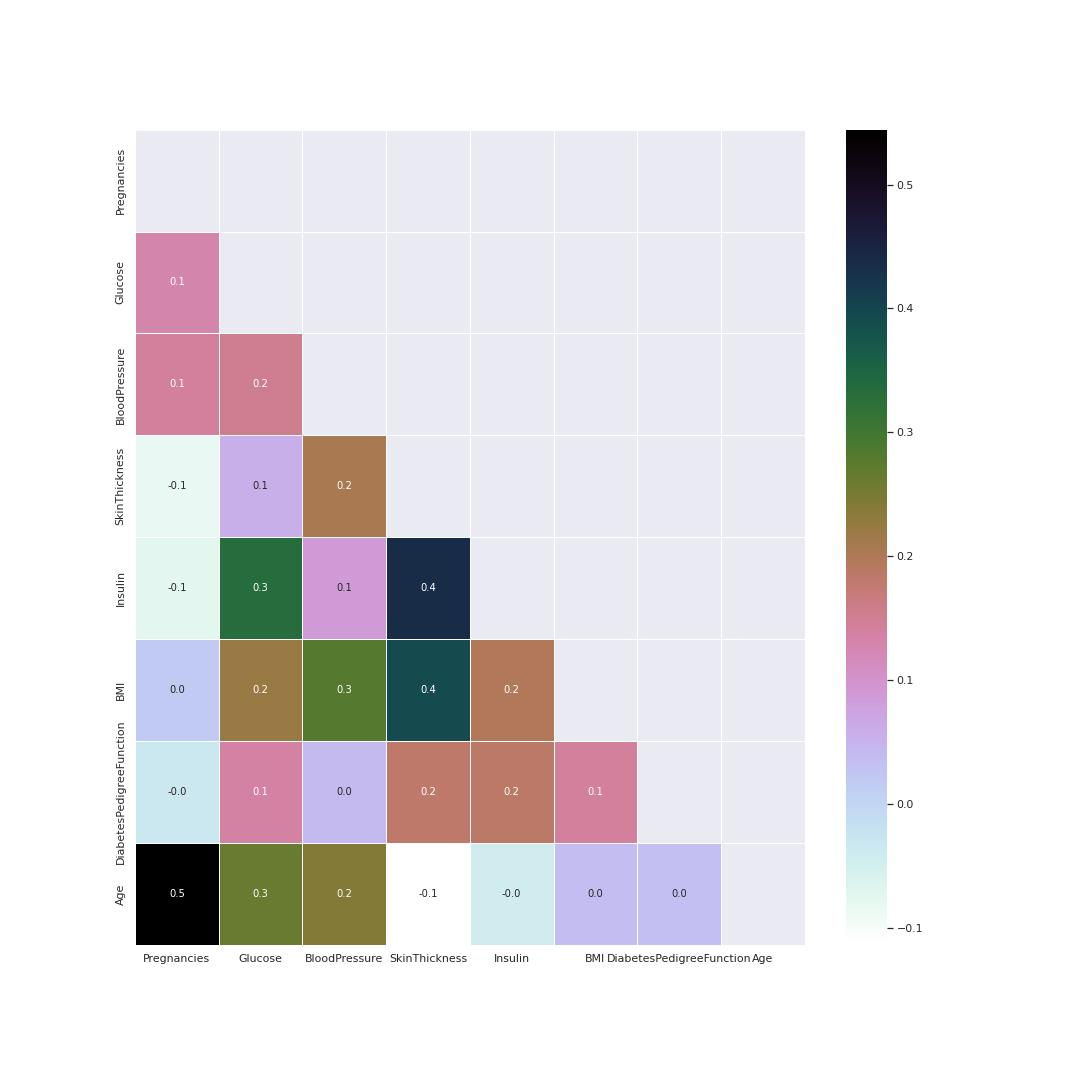
\includegraphics{Corr.jpg}
\caption{Heat map Correlation Coeffi}
\end{figure}

\hypertarget{true-diabetes-distribution}{%
\subsubsection{True Diabetes
Distribution}\label{true-diabetes-distribution}}

To understand data we have to plot data using violin visualization. This
plotting shows where the outcome of diabetes was 1. This shows the
distribution of the diabetes resulting from different factors. This
gives us clear picture that Glucose, BMI and Insulin had the most effect
on the outcome value. This also determines on the data division for
model training and model testing.

\begin{figure}
\centering
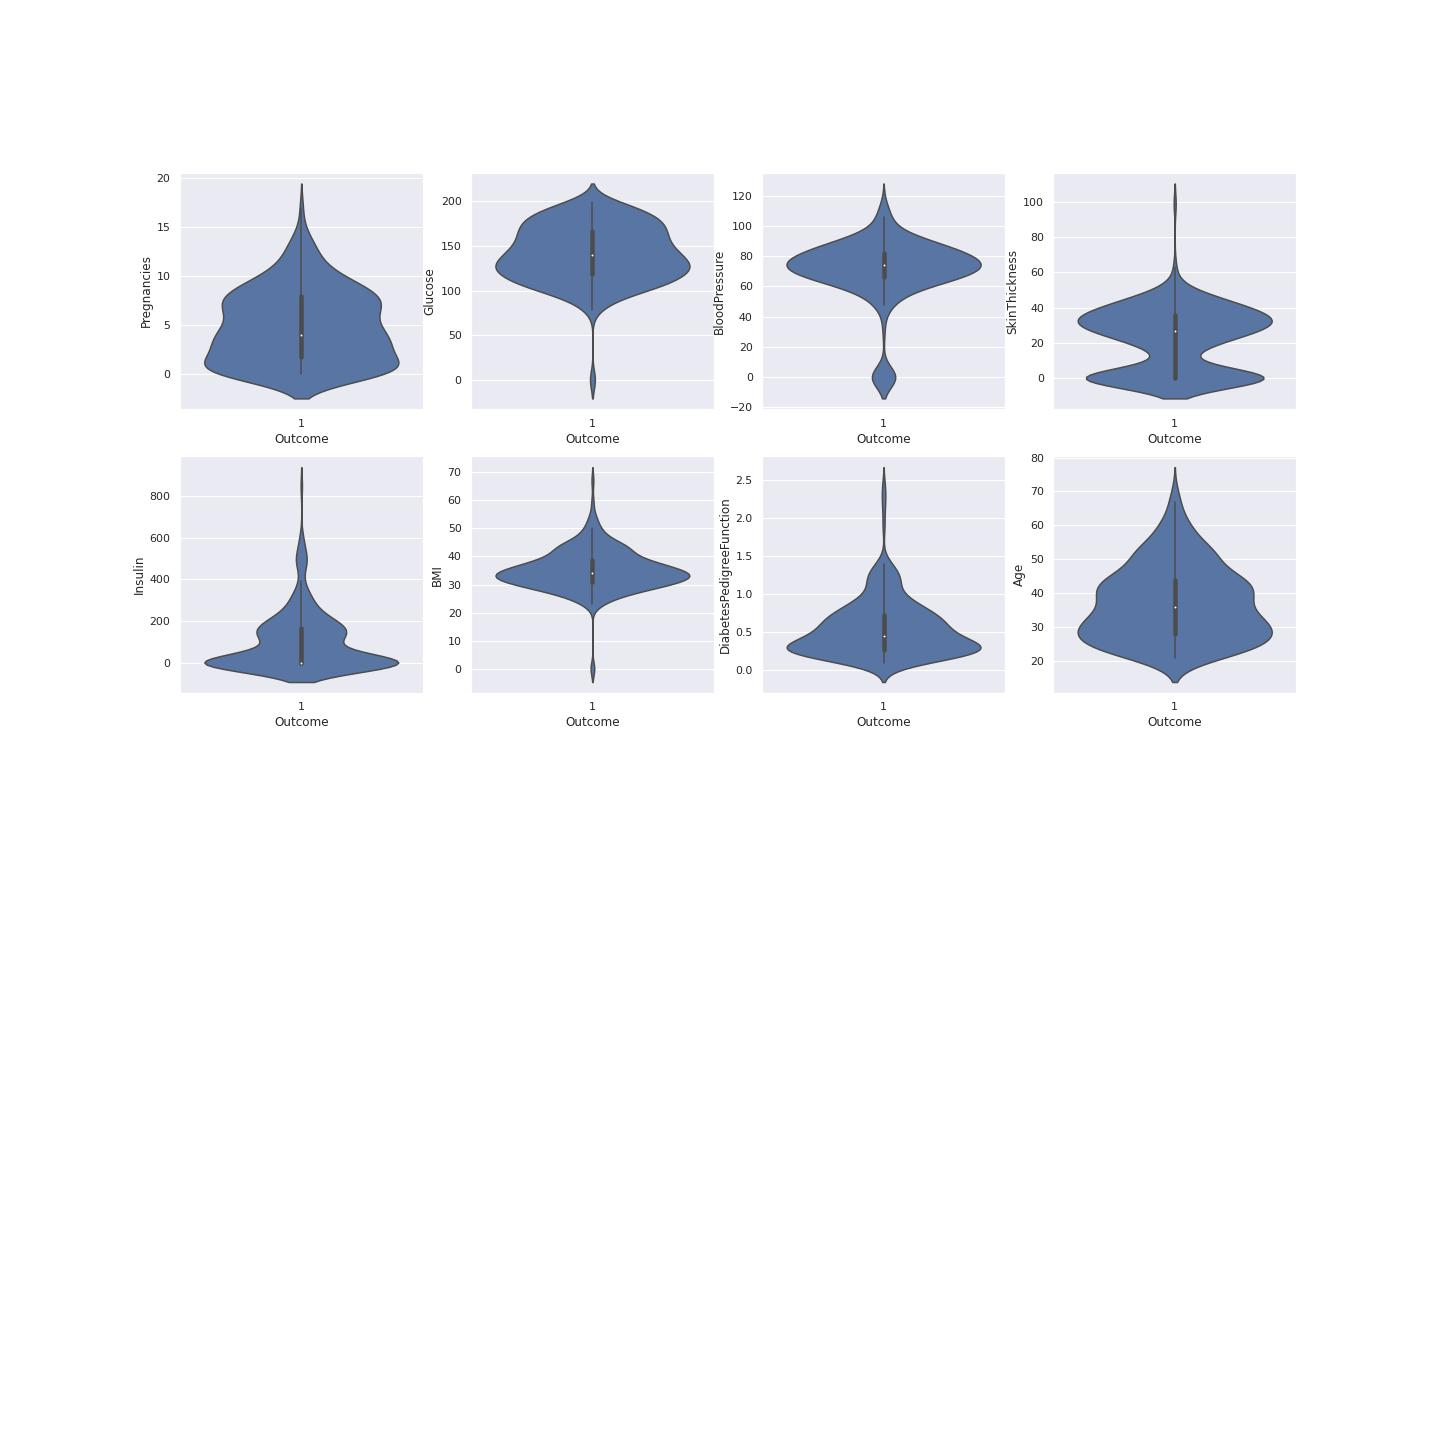
\includegraphics{truediab.jpg}
\caption{True Diabetes}
\end{figure}

\hypertarget{false-diabetes-distribution}{%
\subsubsection{False Diabetes
Distribution}\label{false-diabetes-distribution}}

To understand data we have to plot data using violin visualization. This
plotting shows where the outcome of diabetes was 0.

\begin{figure}
\centering
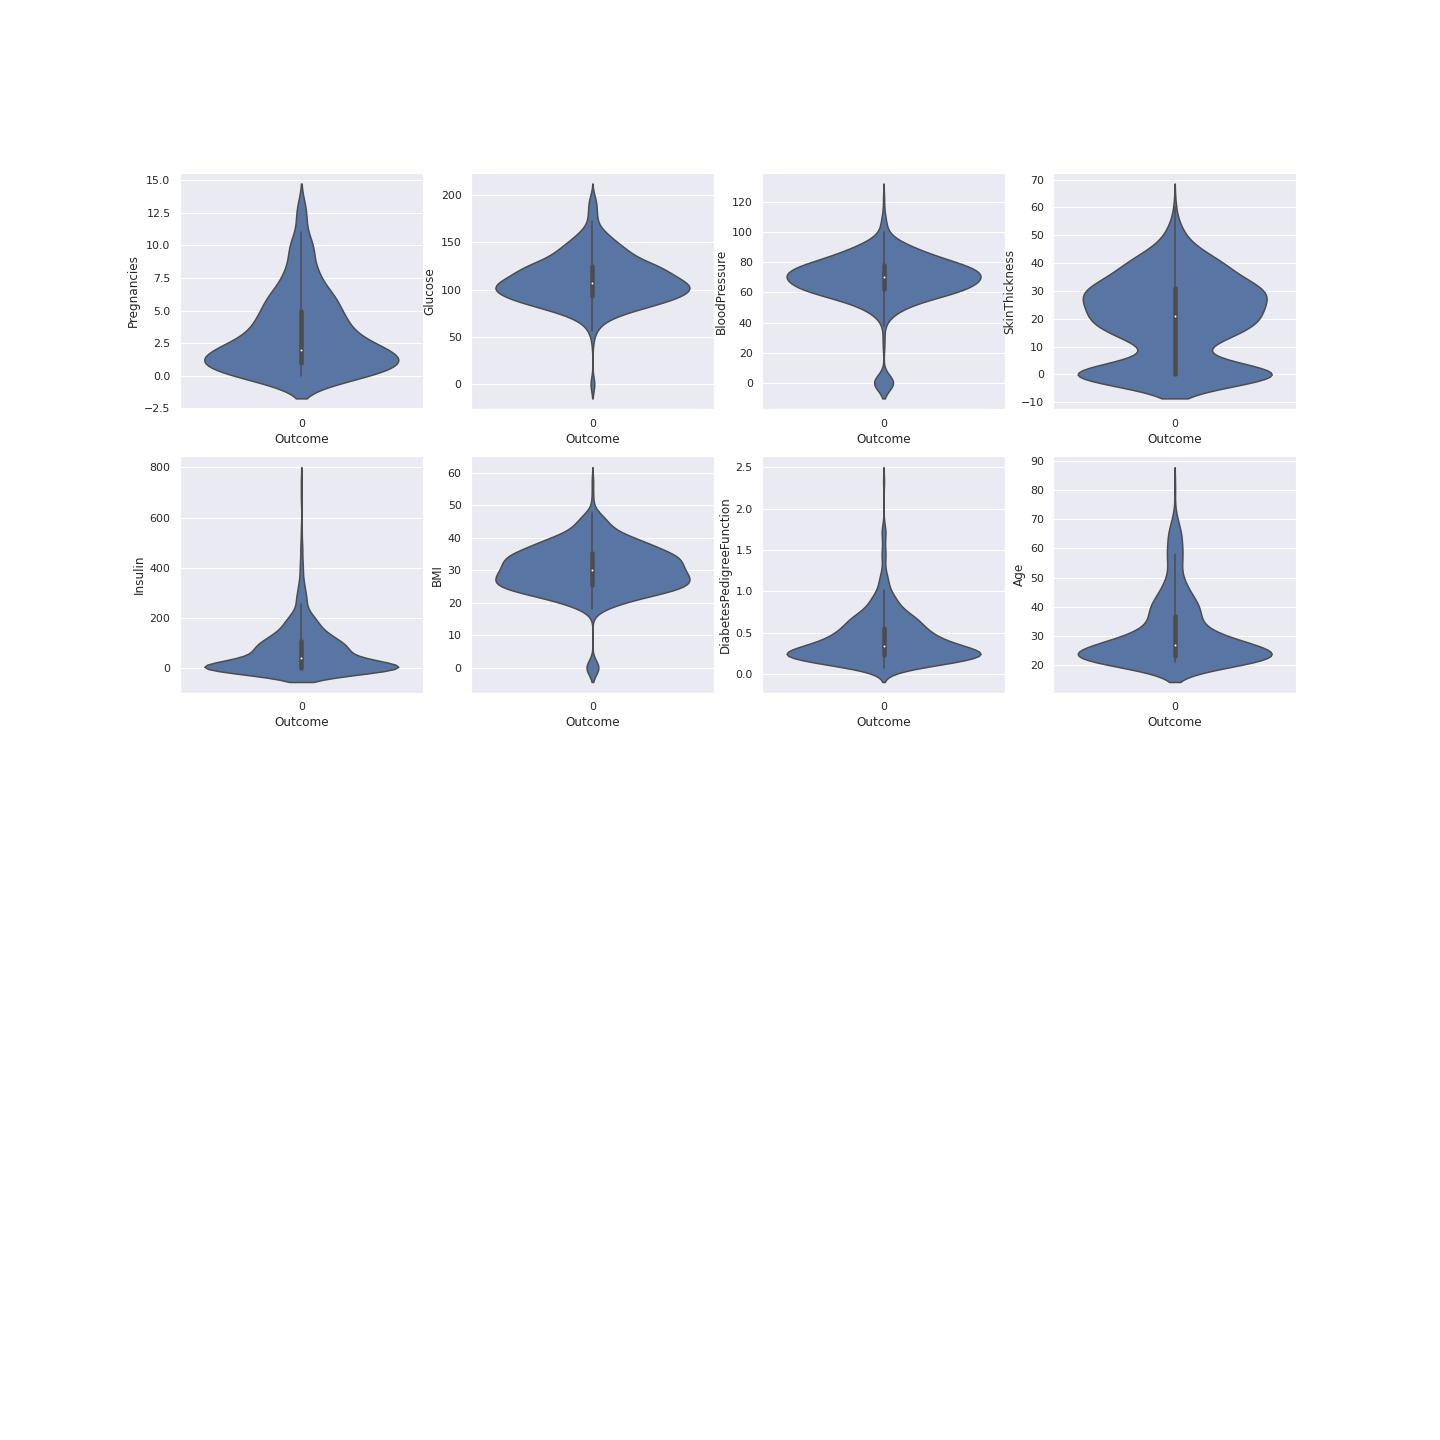
\includegraphics{falsediab.jpg}
\caption{False Diabetes}
\end{figure}

\hypertarget{algorithms-and-techniques}{%
\subsection{Algorithms and Techniques}\label{algorithms-and-techniques}}

\hypertarget{benchmark}{%
\subsection{Benchmark}\label{benchmark}}

\hypertarget{methodology}{%
\section{Methodology}\label{methodology}}

\hypertarget{data-preprocessing}{%
\subsection{Data Preprocessing}\label{data-preprocessing}}

\begin{lstlisting}[language=python]
train = df.sample(frac=0.7, random_state=42)
test = df.drop(train.index)

label = "Outcome"
y_test = test[label]
X_test = test.drop(columns=[label])

\end{lstlisting}

\hypertarget{implementation}{%
\subsection{Implementation}\label{implementation}}

\begin{lstlisting}[language=python]
%%time

predictor = TabularPredictor(label='Outcome', eval_metric='roc_auc',
                             ).fit(train_data=train_s3_path,
                                  time_limit=600,
                                  presets=['best_quality',
                                  'optimize_for_deployment'],
                                )
\end{lstlisting}

\hypertarget{results}{%
\section{Results}\label{results}}

\begin{lstlisting}[language=python]

predictor.fit_summary(show_plot=True)

*** Summary of fit() ***
Estimated performance of each model:
                    model  score_val  pred_time_val    fit_time  pred_time_val_marginal  fit_time_marginal  stack_level  can_infer  fit_order
0     WeightedEnsemble_L2   0.849699       0.910417  242.822065                0.000679           0.457114            2       True          4
1       LightGBMXT_BAG_L1   0.848956       0.067625   41.802209                0.067625          41.802209            1       True          1
2  NeuralNetFastAI_BAG_L1   0.831127       0.364630  104.587116                0.364630         104.587116            1       True          2
3   NeuralNetTorch_BAG_L1   0.830445       0.477483   95.975625                0.477483          95.975625            1       True          3
Number of models trained: 4
Types of models trained:
{'StackerEnsembleModel_TabularNeuralNetTorch', 'WeightedEnsembleModel', 'StackerEnsembleModel_NNFastAiTabular', 'StackerEnsembleModel_LGB'}
Bagging used: True  (with 5 folds)
Multi-layer stack-ensembling used: False 
Feature Metadata (Processed):
(raw dtype, special dtypes):
('float', []) : 2 | ['BMI', 'DiabetesPedigreeFunction']
('int', [])   : 6 | ['Pregnancies', 'Glucose', 'BloodPressure', 'SkinThickness', 'Insulin', ...]
Plot summary of models saved to file: AutogluonModels/ag-20230310_110459/SummaryOfModels.html
*** End of fit() summary ***

\end{lstlisting}

\hypertarget{model-evaluation}{%
\subsection{Model Evaluation}\label{model-evaluation}}

\begin{lstlisting}[language=python]
predictor.evaluate(test_s3_path)

Loaded data from: s3://sagemaker-us-east-1-495962688195/sagemaker/autogluon-tabular/data/test.csv | Columns = 9 / 9 | Rows = 230 -> 230
Evaluation: roc_auc on test data: 0.8274792522424343
Evaluations on test data:
{
    "roc_auc": 0.8274792522424343,
    "accuracy": 0.7478260869565218,
    "balanced_accuracy": 0.6872327940313522,
    "mcc": 0.41186364034362855,
    "f1": 0.5735294117647058,
    "precision": 0.6842105263157895,
    "recall": 0.4936708860759494
}
{'roc_auc': 0.8274792522424343,
 'accuracy': 0.7478260869565218,
 'balanced_accuracy': 0.6872327940313522,
 'mcc': 0.41186364034362855,
 'f1': 0.5735294117647058,
 'precision': 0.6842105263157895,
 'recall': 0.4936708860759494}
\end{lstlisting}

\hypertarget{conclusion}{%
\section{Conclusion}\label{conclusion}}

AutoML frameworks offer an enticing alternative. For the novice, they
remove many of the barriers of deploying high performance ML models. For
the expert, they offer the potential of implementing best ML practices
only once (including strategies for model selection, ensembling,
hyperparameter tuning, feature engineering, data preprocessing, data
splitting, etc.), and then being able to repeatedly deploy them. This
allows experts to scale their knowledge to many problems without the
need for frequent manual intervention

\newpage

\hypertarget{references}{%
\section*{References}\label{references}}
\addcontentsline{toc}{section}{References}

\hypertarget{refs}{}
\begin{CSLReferences}{1}{0}
\leavevmode\vadjust pre{\hypertarget{ref-ehr}{}}%
Aamna. 2023. {``HW1 Machine Learning for EHR.''} Kaggle.
\url{https://kaggle.com/competitions/hw1-machine-learning-for-ehr}.

\leavevmode\vadjust pre{\hypertarget{ref-volo}{}}%
Volodkevich, A. n.d. {``AUC and Its Implementation in CatBoost, Medium.
Towards Data Science.''}
Medium.\href{\%20https://towardsdatascience.com/auc-and-its-implementation-in-catboost-6bc740c01f98\%20(Accessed:\%20March\%2013,\%202023)}{
https://towardsdatascience.com/auc-and-its-implementation-in-catboost-6bc740c01f98
(Accessed: March 13, 2023)}.

\end{CSLReferences}

\end{document}
